\newpage

% \onecolumn

\appendix

\section{Histogramme}
\label{sec:plots}

\begin{figure}[htbp]
  \subfloat[Photomultiplier 1]{
    \label{fig:photomultiplier_1}
    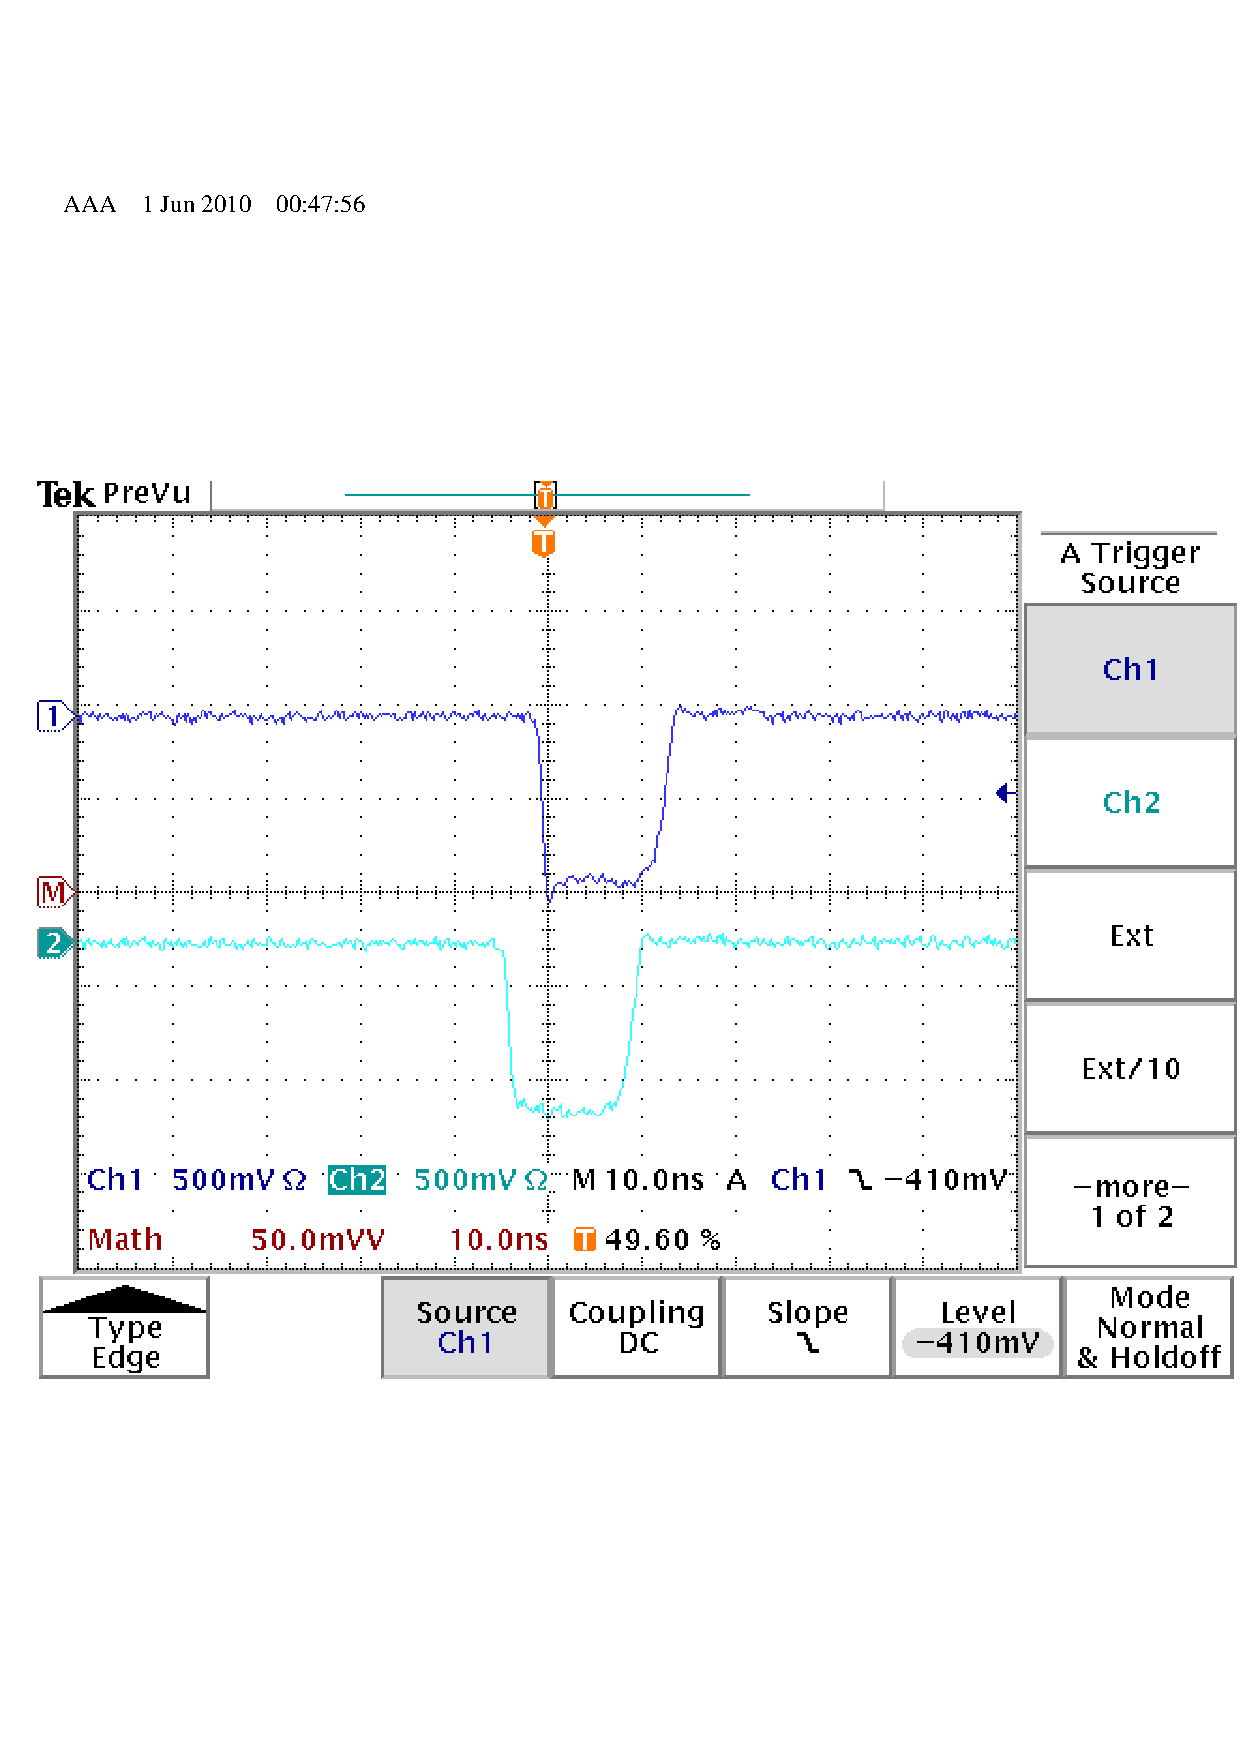
\includegraphics[width=0.445\textwidth,keepaspectratio]{../tmp/TEK00000.pdf}
  }
  \subfloat[Photomultiplier 2]{
    \label{fig:photomultiplier_2}
    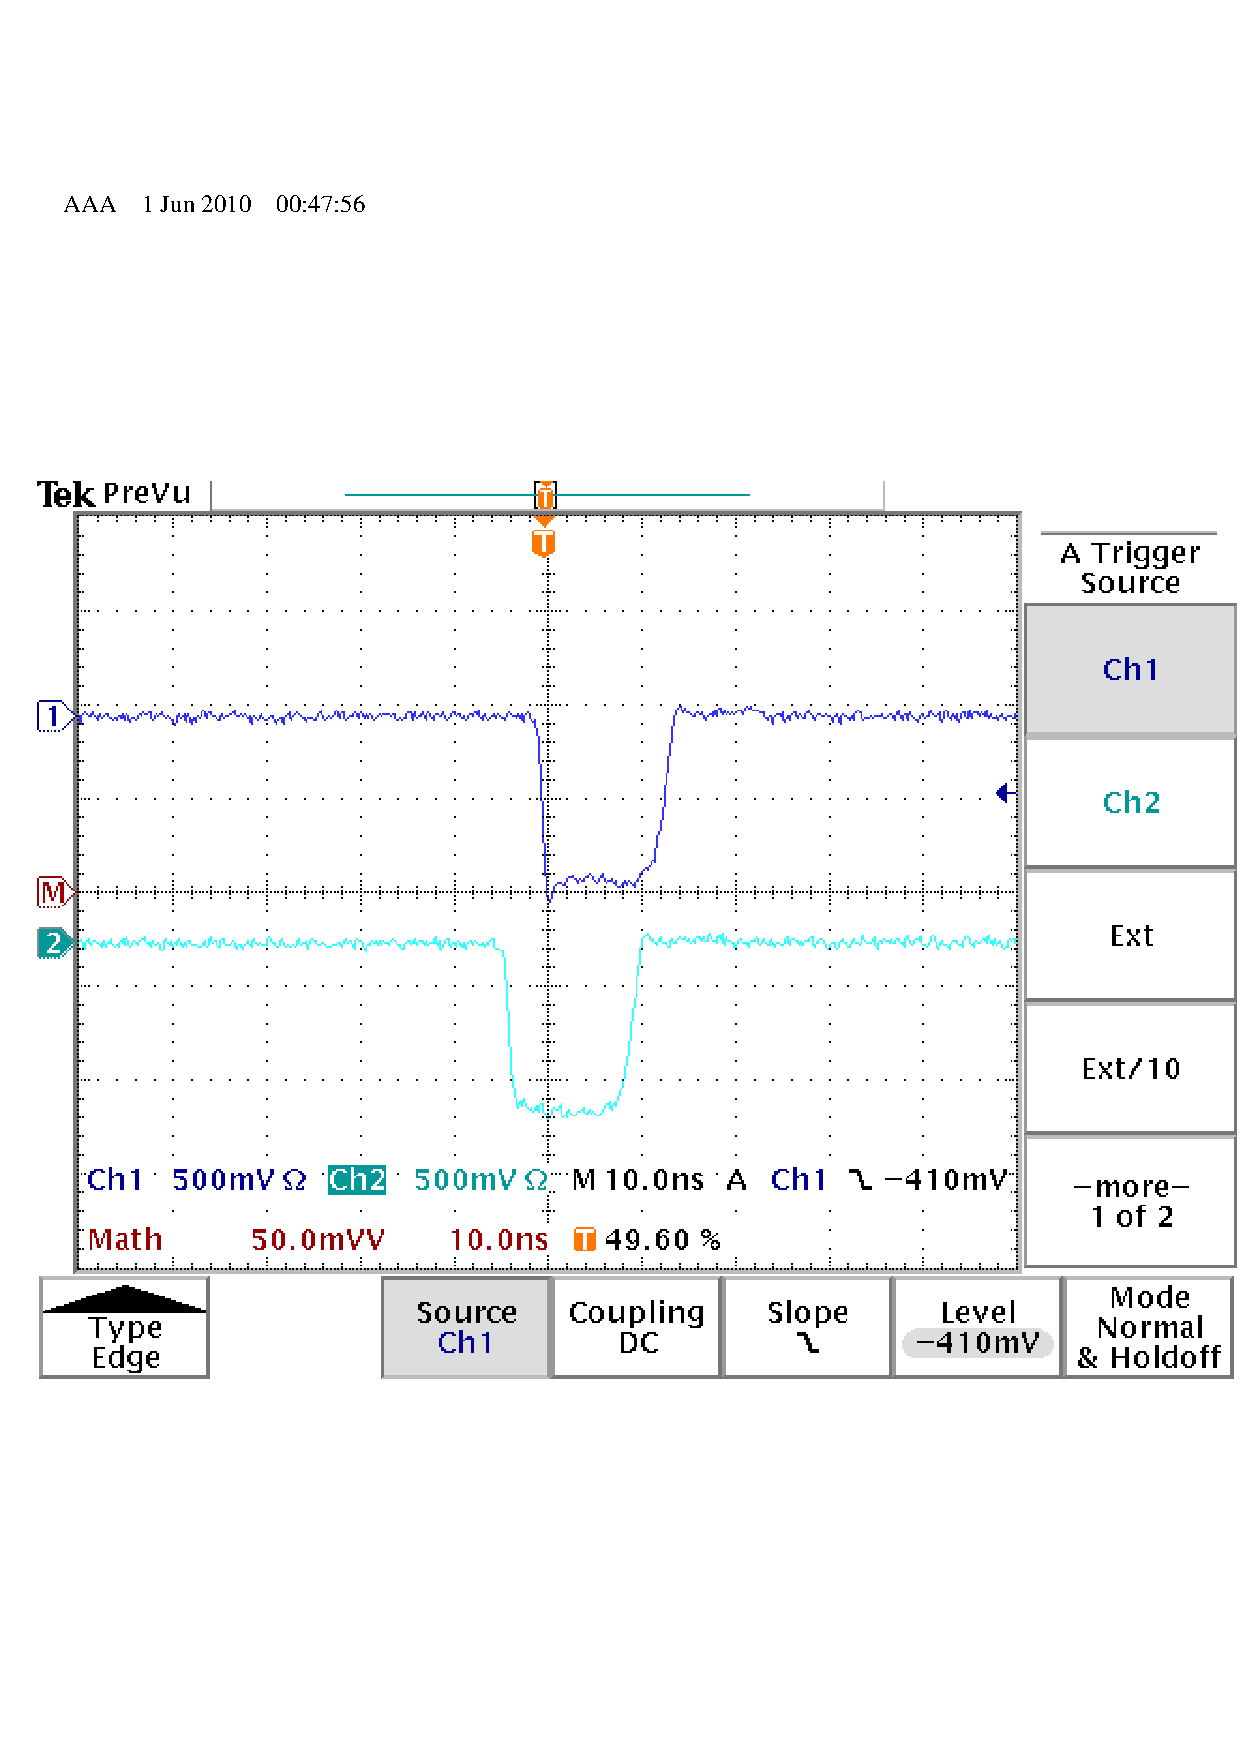
\includegraphics[width=0.445\textwidth,keepaspectratio]{../tmp/TEK00000.pdf}
  }
  \newline
  \subfloat[Photomultiplier 3]{
    \label{fig:photomultiplier_3}
    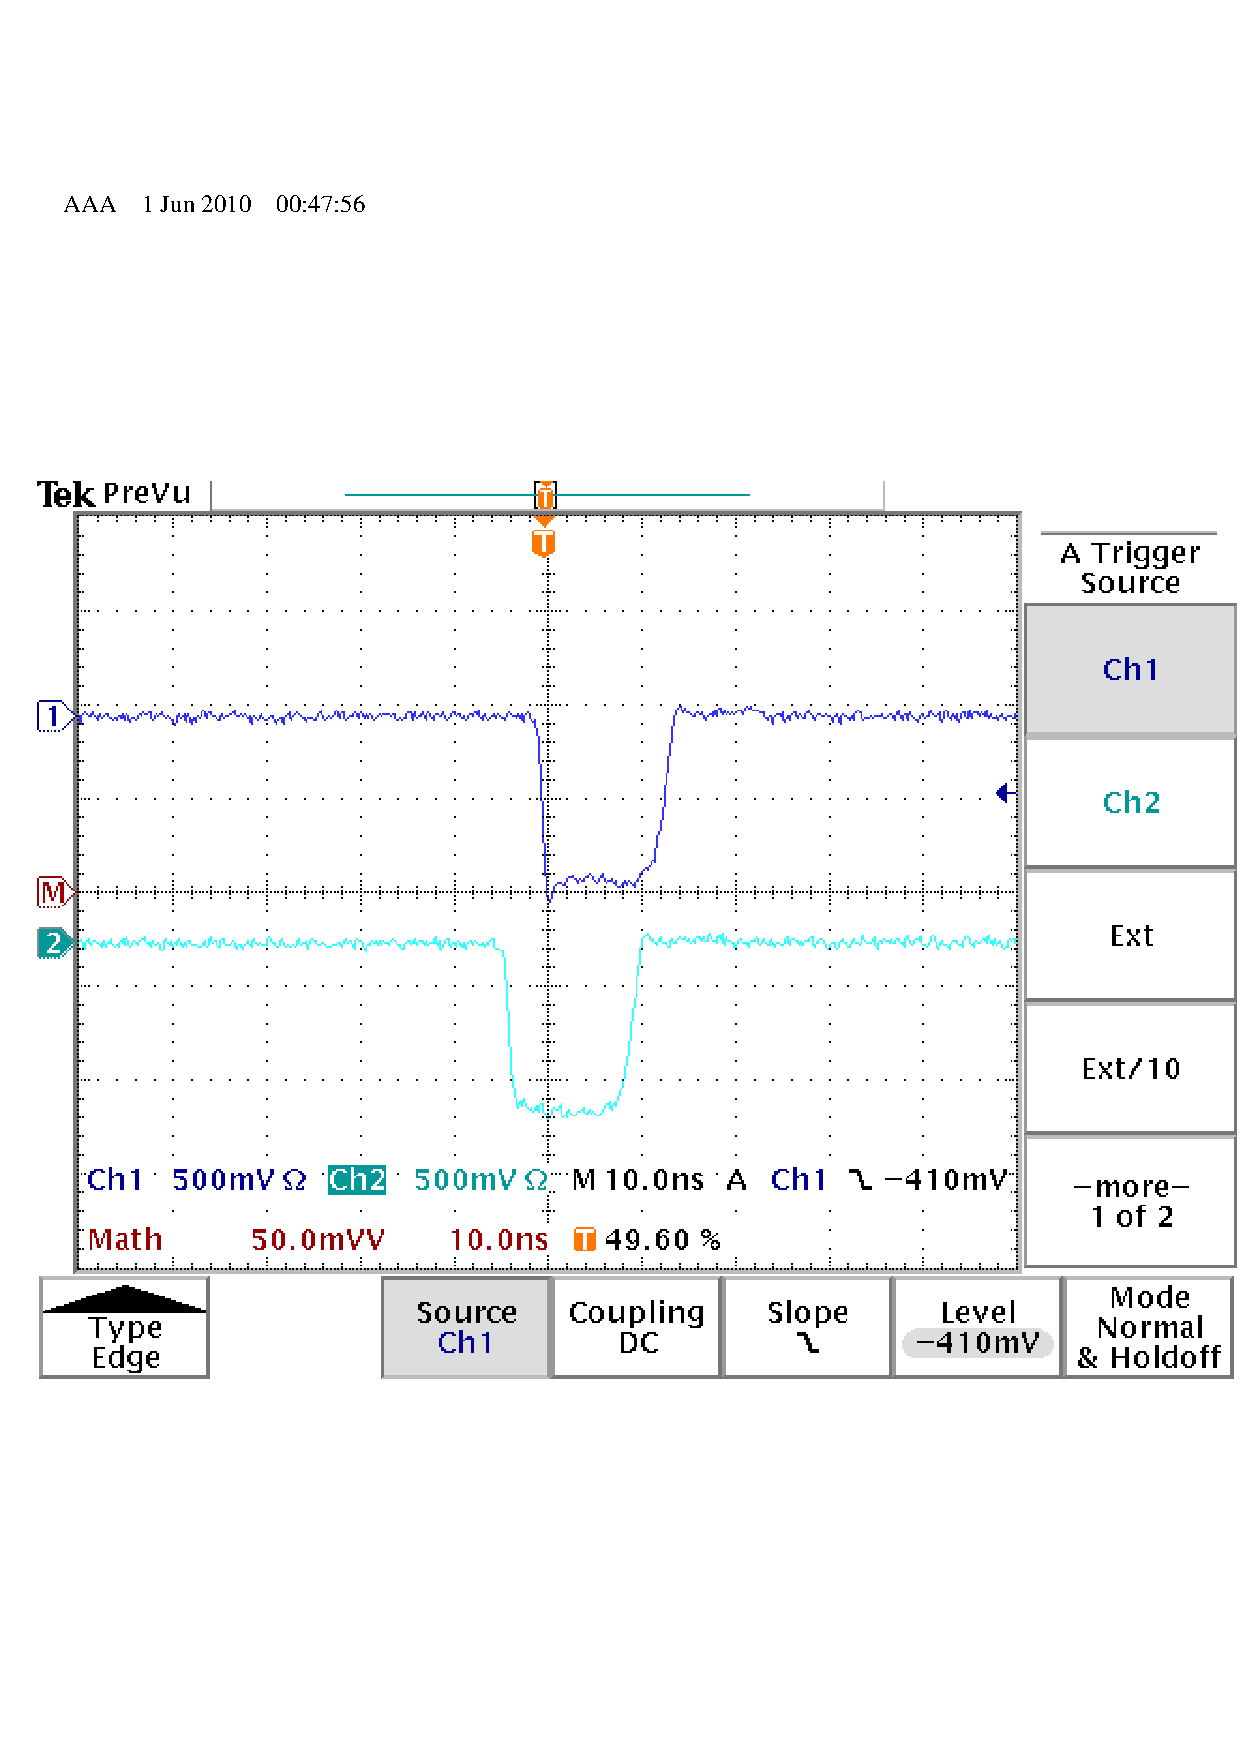
\includegraphics[width=0.445\textwidth,keepaspectratio]{../tmp/TEK00000.pdf}
  }
  \subfloat[Photomultiplier 4]{
    \label{fig:photomultiplier_4}
    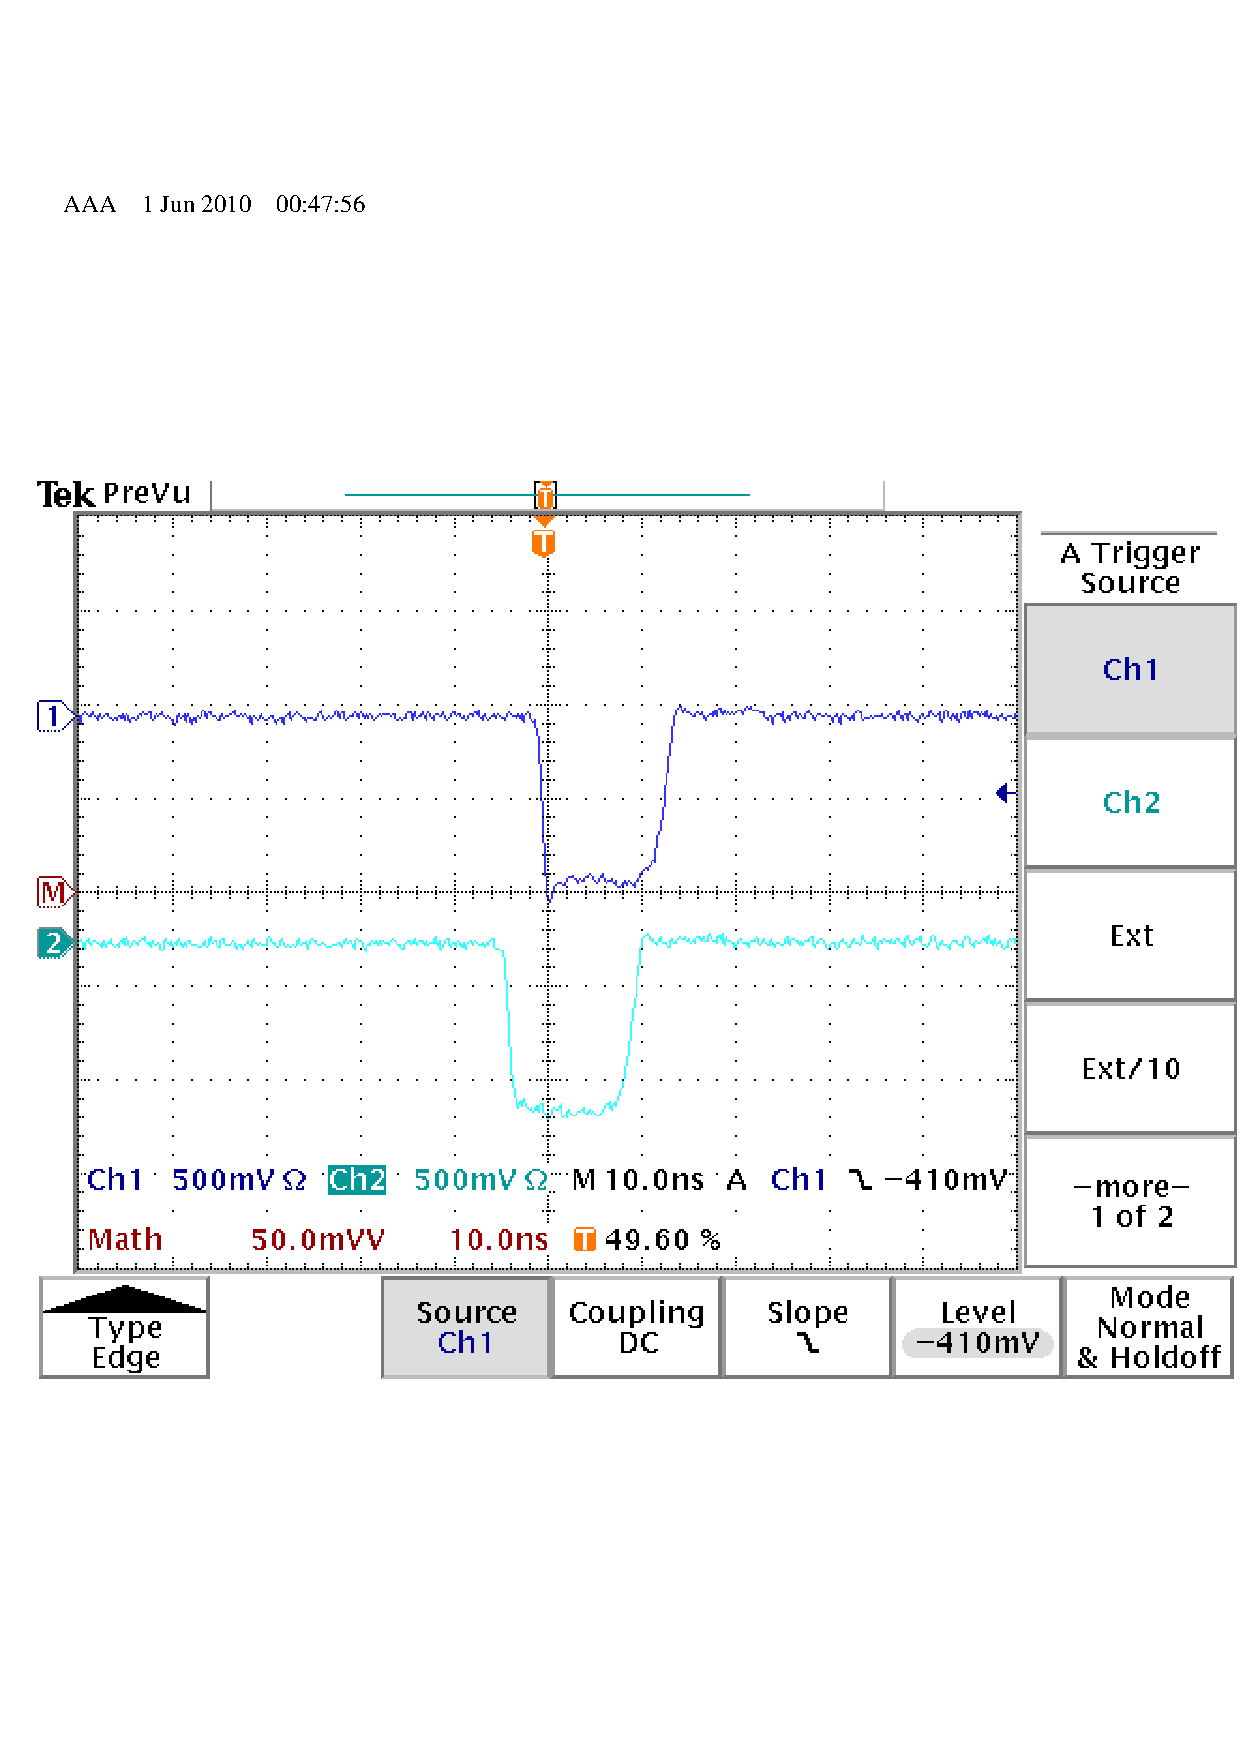
\includegraphics[width=0.445\textwidth,keepaspectratio]{../tmp/TEK00000.pdf}
  }
  \newline
  \subfloat[Photomultiplier 5]{
    \label{fig:photomultiplier_5}
    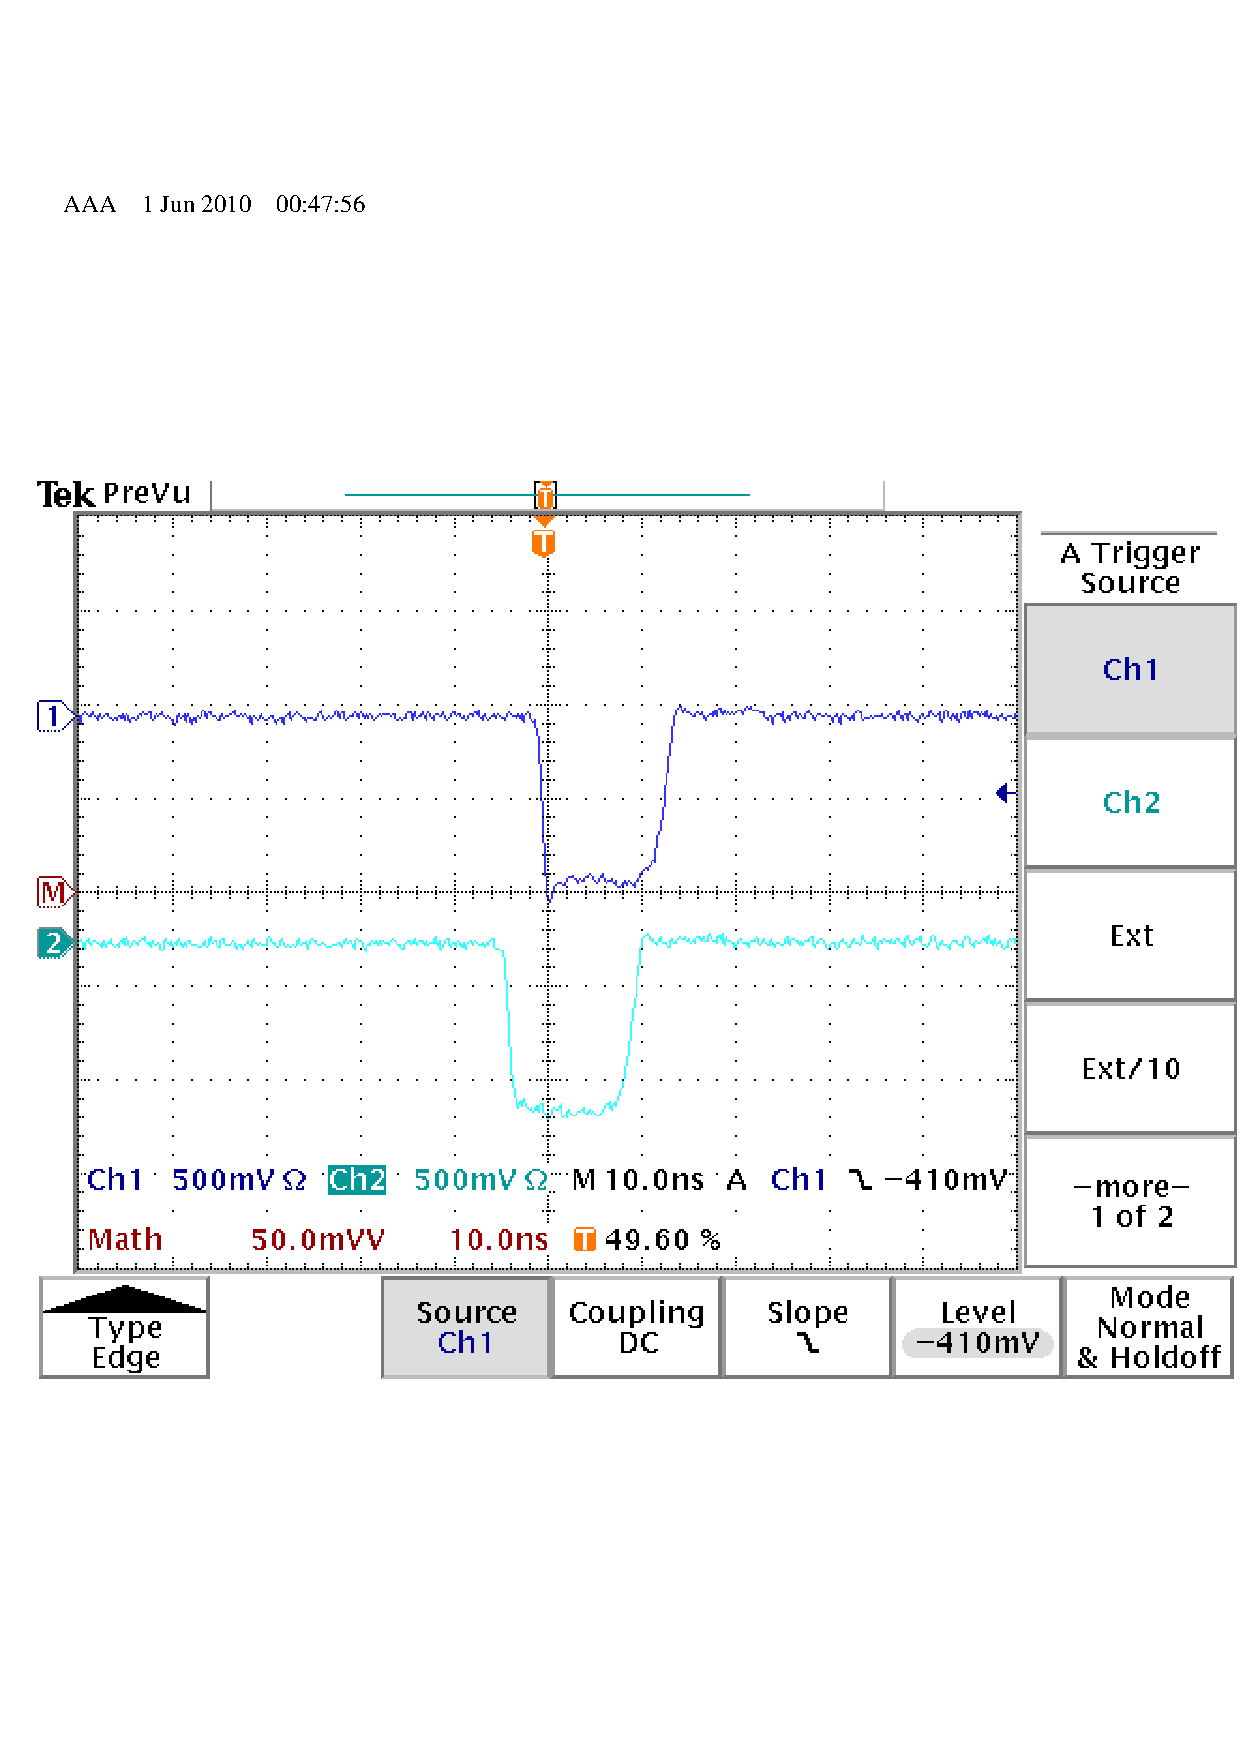
\includegraphics[width=0.445\textwidth,keepaspectratio]{../tmp/TEK00000.pdf}
  }
  \label{fig:PMs}
\end{figure}

\section{Quellcode}

% \lstinputlisting[label=lst:source,caption={Programmquelltext},lastline=248]{
% ../code/main.cpp}
% \lstinputlisting[language=Maxima,label=lst:Berechnungen,
% caption={Berechnungen}]{../code/rechnungen.mac}